\documentclass[11pt,a4paper]{scrartcl}
\usepackage{graphicx}
\usepackage[ngerman]{babel}
\usepackage[utf8]{inputenc}
\usepackage[colorlinks=false,pdfborder={0 0 0}]{hyperref}
\usepackage{longtable}
\usepackage{listings}
\lstset{breaklines=true, breakatwhitespace=true, basicstyle=\small}

\title{Netzwerksicherheit Labor 1\\
	Testen von Firmen-Netzwerken}
\author{Yanick Eberle\\
		Pascal Schwarz}
\date{}
\begin{document}
\maketitle
\newpage
\tableofcontents
\newpage
\section{Aufgabe 1 - Wireshark/ARP}
\subsection{Protokollaufbau}
Die folgende Grafik\footnote{Quelle: http://ipv6.com/images/diagrams/arp1.gif} zeigt den Aufbau des Protokolls.
\begin{figure}[h]
	\centering
	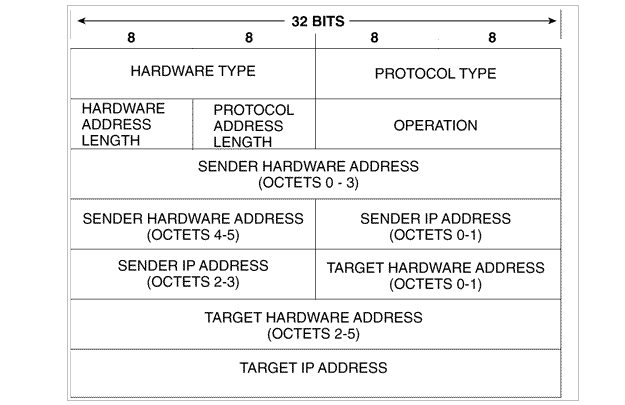
\includegraphics[width=0.7\textwidth]{../aufg1/arp1.png}
	\caption{Address Resolution Protocol}
	\label{fig:arp}
\end{figure}
\subsection{Beantwortung der gestellten Fragen zum Protokoll}
\textbf{Wieviele Bytes ist das ARP Opcode-Feld vom Anfang des Ethernet Frames entfernt?} \\6 Byte\\
\textbf{Welcher Wert hat das Opcode-Feld innerhalb des ARP-payload des Ethernet frame, worin eine ARP Anfrage gestellt ist?} \\ARP request\\
\textbf{Enthält die ARP Meldung die IP Adresse des Senders?} \\Ja\\
\textbf{Wo in der ARP-Anfrage erscheint die "Frage" : Welche Maschine besitzt diese IP Adresse?} \\Operation (Opcode)\\
\textbf{Geben Sie den Inhalt des ARP-Cache Ihres Laptops an, und erklären Sie, was jede
Spalte bedeutet.} \\arp -n\\

\begin{tabular}{l|l|l|l|l|l}
	Address & HWtype & HWaddress & Flags & Mask & Iface \\
	10.196.134.1	&	ether	&	ee:ee:ee:01:07:06	&	C	&	&	eth0 \\
	10.196.134.127	&	ether   &	54:42:49:56:7c:bc	&	C	&	&	eth0
\end{tabular}
\begin{description}
	\item[Address] zu welcher IP gehört der Rest der Information in der Zeile?
	\item[HWType] gibt layer1/2 typ an
	\item[HWAddress] der IP (Spalte 1) zugeordnete Hardwareadresse (hier MAC-Adresse)
	\item[Flags] C steht für Complete (ARP Anfrage abgeschlossen), M wäre permanent, P publish
	\item[Mask] würde zusammen mit publish benutzt
	\item[Iface] über welches Interface ist die HWAddr erreichbar
\end{description}


\newpage
\section{Aufgabe 2 - Utilities ping, hping3, dig, traceroute}
\subsection{Perl Script für Host-Discovery im Subnet}
\lstinputlisting[numbers=left]{../aufg2/netscan.pl}

Das Script erzeugt eine Ausgabe ähnlich der Folgenden:
\begin{lstlisting}
10.196.134.1
10.196.134.16
10.196.134.17
10.196.134.19
10.196.134.21
10.196.134.118
10.196.134.120
\end{lstlisting}

\subsection{DNS Protokoll}
Viele Informationen in diesem Abschitt stammen von \url{http://doc-tcpip.org/Dns/named.dns.message.html}.
\subsubsection{DNS-Request Packet: Welches Protokoll wird benutzt? Welche Vorteile bietet
dies für einen DNS?}
Es wird UDP als Transportprotokoll (siehe Grafik \ref{fig:dns_2_2_1} auf Seite \pageref{fig:dns_2_2_1}) eingesetzt. Dadurch entsteht weniger Overhead (hauptsächlich weil kein 3-way-Handshake nötig ist), was wiederum die Performance erhöht (geringere Latenz).
\begin{figure}[h]
	\centering
	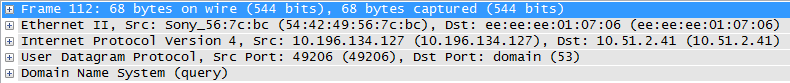
\includegraphics[width=1.0\textwidth]{../aufg2/dns_2_2_1.png}
	\caption{DNS Anfrage in Wireshark}
	\label{fig:dns_2_2_1}
\end{figure}

\subsubsection{DNS-Request Paket: Welcher src und dst port werden definiert? Wie interpretieren Sie das Resultat?}
Auf Zielhost wird auf Port 53 abgehört. Da es eine Anfrage ist, ist der Destination Port 53. Siehe hierzu Grafik \ref{fig:dns_2_2_2} auf Seite \pageref{fig:dns_2_2_2}.
\begin{figure}[h]
	\centering
	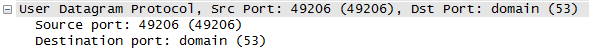
\includegraphics[width=1.0\textwidth]{../aufg2/dns_2_2_2.png}
	\caption{DNS Ports in Wireshark}
	\label{fig:dns_2_2_2}
\end{figure}

\subsubsection{DNS-Response Paket: Welche Felder gibt es? Erklären Sie deren Bedeutung.}
\begin{description}
	\item[Time] Antwortzeit
	\item[Transaction ID] eindeutige Nummer, muss mit Transaction ID des DNS Requests übereinstimmen, ist dies nicht der Fall, muss die Antwort verworfen werden.
	\item[Flags] Request, Response, Error, no Error, \ldots
	\item[Questions] Anzahl Anfragen
	\item[Answer RRs] Anzahl Antworten
	\item[Authority RRs] RRs, die auf verantwortliche Server deuten
	\item[Additional RRs] RRs mit weiteren Informationen/Records
\end{description}
\textbf{RR} steht hier für \textbf{Resource Record}, ein Format zur Angabe des Mappings von IP-Adresse zu Name bzw. umgekehrt - oder weitere Information. Resource Records sind die Einträge in den Datenbank-Files des Name Servers.
\begin{figure}[h]
	\centering
	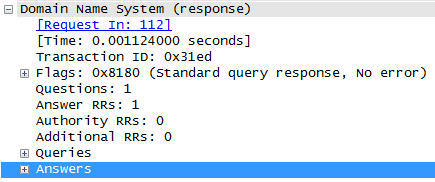
\includegraphics[width=0.7\textwidth]{../aufg2/dns_2_2_3.png}
	\caption{Header in DNS Response}
	\label{fig:dns_2_2_3}
\end{figure}

\subsubsection{DNS-Response Paket: Was enthält das Feld Answer? Erklären Sie jede zusätzliche
Information, die Sie in diesem Feld gefunden haben.}
\begin{description}
	\item[NAME] Der Domain-Name, zu der dieser RR gehört. 
	\item[TYPE] Der RR-Typ Code. Spezifiziert die Bedeutung des Feldes RDATA. Zwei Oktets. 
	\item[CLASS] RR-Klasse. Spezifiziert die Bedeutung des Feldes RDATA. Zwei Oktets. 
	\item[TTL] Time To Live - eine 32-bittige Zahl, die die Anzahl der Sekunden angibt, für die man diesen Record im Cache behalten darf. Null bedeutet, das dieser RR nur für die aktuelle Transaktion gilt. 
	\item[RDLENGTH] Eine 16-bittige Zahl, die die Anzahl der Oktets im RDATA Feld angibt. 
	\item[RDATA] Ein String variabler Länge (Oktets), der die Resource beschreibt. Das Format hängt von den Setzungen in TYPE und CLASS ab. Bei TYPE = A und CLASS = IN wäre das also eine normale 4 Oktet (32-bittige) ARPA Internet Adresse.
\end{description}
\begin{figure}[h]
	\centering
	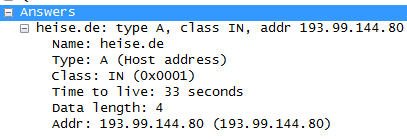
\includegraphics[width=0.7\textwidth]{../aufg2/dns_2_2_4.png}
	\caption{Answer-Abschnitt einer Response}
	\label{fig:dns_2_2_4}
\end{figure}

\subsection{Traceroute apple.com}
Die geographische Lage der Router kann insbesondere in diesem Beispiel über die reverse DNS Einträge festgelegt werden. So ist beispielsweise *.zrh1.he.net in Zürich. Der Sprung passiert folglich zwischen Hop 13 und 14, also zwischen Amsterdam und Washington.

Grundsätzlich sollte der Sprung an der Latenzzeit ersichtlich sein. In diesem Fall ist die Latenzzeit der Router in Frankfurt und Amsterdam jedoch schon sehr hoch, was ev. auf eine Überlastung am Übergang zwischen he.net und xo.net in Frankfurt (am DE-CIX) zurückzuführen ist.
\begin{figure}[h]
	\centering
	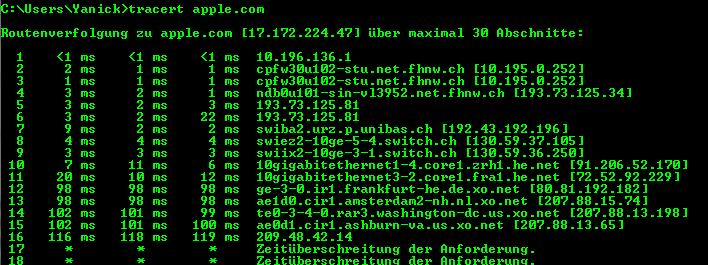
\includegraphics[width=1.0\textwidth]{../aufg2/tracert_apple.png}
	\caption{Traceroute zu apple.com}
	\label{fig:traceroute_apple}
\end{figure}

\newpage
\section{Aufgabe 3 - Nmap/Wireshark}
Wir haben den Aufruf folgendermassen gemacht: \begin{verbatim}nmap -P0 -p80 www.fhnw.ch\end{verbatim} Wir haben die Option -P0 gesetzt, weil wir wissen, dass unter www.fhnw.ch (mindestens) ein Server erreichbar ist. Der Output des Commands war der folgende:

\begin{lstlisting}
Starting Nmap 6.01 ( http://nmap.org ) at 2012-11-15 08:18 CET
Nmap scan report for www.fhnw.ch (147.86.3.160)
Host is up (0.0021s latency).
rDNS record for 147.86.3.160: wsnmu25.fhnw.ch
PORT   STATE SERVICE
80/tcp open  http
Nmap done: 1 IP address (1 host up) scanned in 0.03 seconds
\end{lstlisting}

Mit dem Output können wir praktisch den gesamten aufgezeichneten Verkehr (siehe Grafik \ref{fig:traffic_nmap-p80} auf Seite \pageref{fig:traffic_nmap-p80} begründen:
\begin{itemize}
	\item Der Name muss zu einer IP (hier 147.86.3.160) aufgelöst werden, was mittels DNS geschieht.
	\item Die IP wird zurück zu einem Namen aufgelöst (reverse DNS Lookup, "rDNS record..."), ebenfalls via DNS.
	\item Danach wird ein kompletter TCP-3-way-Handshake durchgeführt und die Verbindung danach sofort wieder beendet (Frame 8 mit TCP Flags RST,ACK).
	\item Da der TCP-Handshake erfolgreich durchgeführt werden konnte zeigt uns nmap an, dass der Port geöffnet ist.
\end{itemize}

\begin{figure}[h]
	\centering
	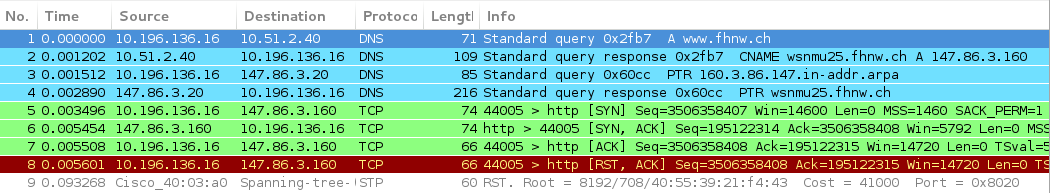
\includegraphics[width=1.0\textwidth]{../aufg3/traffic_nmap-p80.png}
	\caption{Datenverkehr, der durch den nmap-Aufruf ausgelöst wurde}
	\label{fig:traffic_nmap-p80}
\end{figure}

\newpage
\section{Aufgabe 4 - Installation Metasploit}
Metaplsploit wurde unter Arch Linux mithilfe des Pakets von \url{https://aur.archlinux.org/packages.php?ID=2880} installiert. Das Package beinhaltet Postgresql nicht, daher musste dieser Datenbankdienst separat über die Paketverwaltung installiert und danach konfiguriert werden. Die Administration von Postgresql wurde mit dem Paket pgadmin abgewickelt (Erstellen eines Benutzers und einer Datenbank).
Nach diesen Schritten wurde metasploit folgendermassen fertig eingerichtet:
\begin{lstlisting}
$ sudo msfupdate
$ gem install pg
$ msfconsole
msf > db_connect metasploit:****@127.0.0.1/metasploit
\end{lstlisting}
Nach diesen Schritten ist metasploit bereit für Scans und mit der Datenbank verbunden.


\newpage
\section{Aufgabe 5 - Footprinting/Scanning}
\subsection{Footprinting}
\subsubsection{Whois fhnw.ch}
\begin{lstlisting}
Domain name:
fhnw.ch

Holder of domain name:
Fachhochschule Nordwestschweiz FHNW
Graf Heinz
ICT Kommunikation
Steinackerstrasse 5
CH-5210 Windisch
Switzerland
Contractual Language: German

Technical contact:
Fachhochschule Nordwestschweiz FHNW
Graf Heinz
ICT Kommunikation
Steinackerstrasse 5
CH-5210 Windisch
Switzerland

DNSSEC:N

Name servers:
ns.inwx.de
ns1.fhnw.ch [147.86.3.20]
ns2.fhnw.ch [147.86.3.21]
\end{lstlisting}

\subsubsection{DNS Einträge}
\begin{figure}[p]
	\centering
	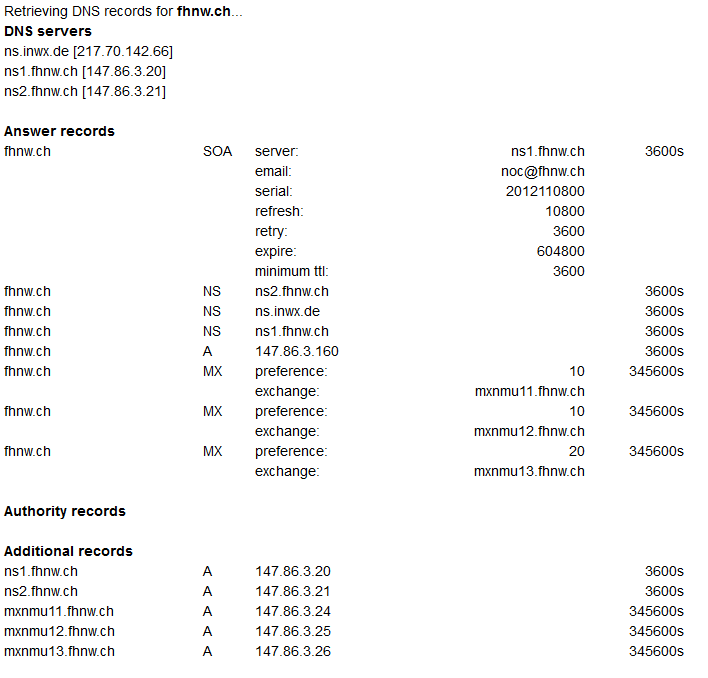
\includegraphics[width=0.6\textwidth]{../aufg5/dns_records.png}
	\caption{DNS Einträge fhnw.ch}
	\label{fig:dns_records}
\end{figure}

\subsubsection{Infos zur Website}
Die Informationen in Grafik \ref{fig:website_infos} auf Seite \pageref{fig:website_infos} stammen von \url{http://www.websitelibrary.ch/fhnw.ch}.
\begin{figure}[p]
	\centering
	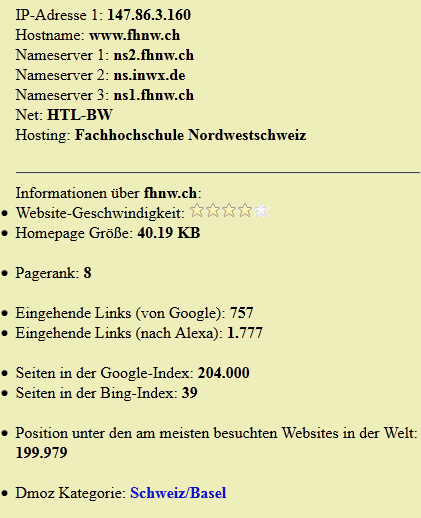
\includegraphics[width=0.5\textwidth]{../aufg5/website_infos.png}
	\caption{Informationen zu www.fhnw.ch}
	\label{fig:website_infos}
\end{figure}

\subsubsection{Informationen zu Mail und Netzwerk}
Eberle: Quellenangabe hier bitte - Grafik \ref{fig:iprange_infos} auf Seite \pageref{fig:iprange_infos}
\begin{figure}[p]
	\centering
	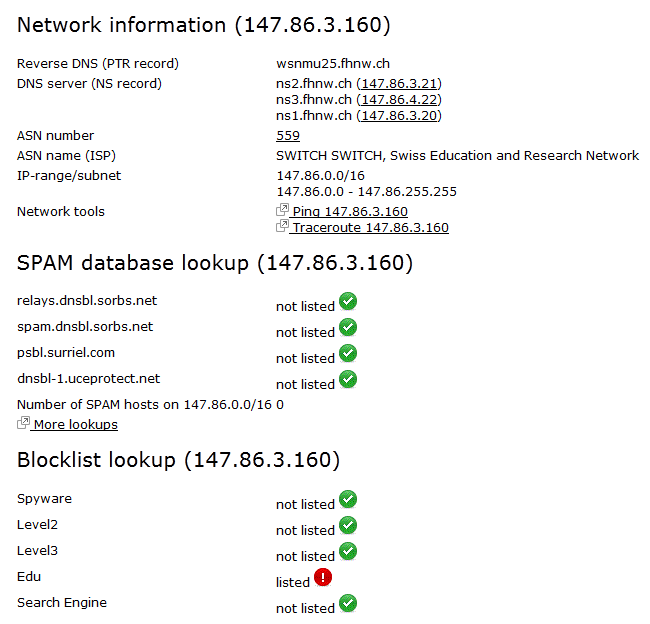
\includegraphics[width=0.6\textwidth]{../aufg5/iprange_infos.png}
	\caption{Informationen zu Mail und Netzwerk}
	\label{fig:iprange_infos}
\end{figure}

\subsubsection{Informationen zum Leiter Netzwerkteam}
Die Grafik \ref{fig:heinz_graf1} auf Seite \pageref{fig:heinz_graf1} zeigt die Informationen über Heinz Graf auf der FHNW-Website.

Gemäss \url{http://www.bienen-ag.ch/index.php?option=com_content&view=article&id=193} ist er auch Beisitzer im Verband Aargauischer Bienenzüchtervereine.
\begin{figure}[p]
	\centering
	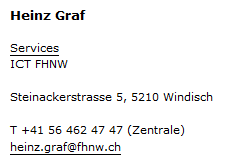
\includegraphics[width=0.4\textwidth]{../aufg5/heinz_graf1.png}
	\caption{Informationen zu Heinz Graf von der FHNW Website}
	\label{fig:heinz_graf1}
\end{figure}

\subsubsection{Via Google gefundene Informationen}
Die Anfrage \textbf{site:fhnw.ch} lieferte u.A. die folgenden Treffer:
\begin{lstlisting}
www.fhnw.ch/
www0.fhnw.ch
web.fhnw.ch/
webtransfer.fhnw.ch/
weblogin.fhnw.ch
webmail.fhnw.ch
sapportal.fhnw.ch/
pms.fhnw.ch/
www.students.fhnw.ch/
webcorp2.fhnw.ch/
blogs.fhnw.ch
eranger.fhnw.ch/
es.fhnw.ch/
aai-logon.fhnw.ch
helio.i4ds.technik.fhnw.ch
tools.fhnw.ch
www.ph.fhnw.ch
portfolio-kompetenzmanagement.fhnw.ch
mediothek.hgk.fhnw.ch/
status.fhnw.ch
ict.campus-brugg-windisch.fhnw.ch
pensentool.fhnw.ch
genius.wirtschaft.fhnw.ch
m.fhnw.ch
*.imvs.technik.fhnw.ch/
*.cs.technik.fhnw.ch/
\end{lstlisting}
Mit \textbf{link:fhnw.ch} konnten folgende Einträge gefunden werden:
\begin{lstlisting}
www.unilu.ch/deu/links_4006.html
lib.consortium.ch/html_wrapper.php?dir=libraries&src=addresses1
www.kgv.ch/links
www.swissdigin.ch/apps/swissdigin.nsf/de/leitfaeden
www.i4ds.ch/team.html
www.esski.ch/
www.ftal.net/UEber-uns.73.0.html
www.esbasel.ch/en/impressum/
\end{lstlisting}

\subsubsection{Reverse-DNS-Namen von 147.86.0.0/16}
In der folgenden Tabelle sind die PTR-Einträge im DNS für die externe IP-Range der FHNW gelistet.
\begin{longtable}{p{2.5cm}|p{7cm}}
	\textbf{IP Adresse} & \textbf{PTR-Eintrag} \\
	\endfirsthead
	\textbf{IP Adresse} & \textbf{PTR-Eintrag} \\
	\endhead
	\multicolumn{2}{l}{\textit{Fortführung auf nächster Seite\ldots}} \\
	\endfoot
	\endlastfoot
	147.86.3.160 & wsnmu25.fhnw.ch \\
	147.86.3.161 & wsnmu25-sec1.fhnw.ch \\
	147.86.3.162 & wsnmu25-sec2.fhnw.ch \\
	147.86.3.163 & wsnmu25-sec3.fhnw.ch \\
	147.86.3.164 & wsnmu32.fhnw.ch \\
	147.86.3.165 & wsnmu32-sec1.fhnw.ch \\
	147.86.3.166 & wsnmu32-sec2.fhnw.ch \\
	147.86.3.167 & wsnmu32-sec3.fhnw.ch \\
	147.86.3.168 & wsnmu32-sec4.fhnw.ch \\
	147.86.3.169 & wsnmu32-sec5.fhnw.ch \\
	147.86.3.170 & wsnmu31.fhnw.ch \\
	147.86.3.171 & wsnmu31-sec1.fhnw.ch \\
	147.86.3.172 & wsnmu31-sec2.fhnw.ch \\
	147.86.3.173 & wsnmu31-sec3.fhnw.ch \\
	147.86.3.174 & wsnmu31-sec4.fhnw.ch \\
	147.86.3.175 & wsnmu31-sec5.fhnw.ch \\
	147.86.3.176 & wsnmu33.fhnw.ch \\
	147.86.3.177 & wsnmu33-sec1.fhnw.ch \\
	147.86.3.178 & wsnmu33-sec2.fhnw.ch \\
	147.86.3.179 & wsnmu33-sec3.fhnw.ch \\
	147.86.3.180 & wsnmu33-sec4.fhnw.ch \\
	147.86.3.182 & wsnmu14.fhnw.ch \\
	147.86.3.183 & wsnmu37.fhnw.ch \\
	147.86.3.184 & wsnmu37-sec1.fhnw.ch \\
	147.86.3.185 & wsnmu37-sec2.fhnw.ch \\
	147.86.3.186 & wsnmu37-sec3.fhnw.ch \\
	147.86.3.187 & wsnmu37-sec4.fhnw.ch \\
	147.86.3.188 & wsnmu37-sec5.fhnw.ch \\
	147.86.3.189 & wsnmu37-sec6.fhnw.ch \\
	147.86.3.190 & wsnmu37-sec7.fhnw.ch \\
	147.86.3.191 & wsnmu37-sec8.fhnw.ch \\
	147.86.3.200 & wsnmu33-sec10.fhnw.ch \\
	147.86.3.201 & wsnmu33-sec11.fhnw.ch \\
	147.86.3.202 & wsnmu33-sec12.fhnw.ch \\
	147.86.3.203 & wsnmu33-sec13.fhnw.ch \\
	147.86.3.204 & wsnmu33-sec14.fhnw.ch \\
	147.86.3.205 & wsnmu33-sec15.fhnw.ch \\
	147.86.3.206 & wsnmu33-sec16.fhnw.ch \\
	147.86.3.207 & wsnmu33-sec17.fhnw.ch \\
	147.86.3.208 & wsnmu33-sec18.fhnw.ch \\
	147.86.3.209 & wsnmu33-sec19.fhnw.ch \\
	147.86.3.210 & wsnra111.fhnw.ch \\
	147.86.3.211 & wsnra111-sec1.fhnw.ch \\
	147.86.3.212 & wsnra111-sec2.fhnw.ch \\
	147.86.3.213 & wsnra111-sec3.fhnw.ch \\
	147.86.3.214 & wsnra111-sec4.fhnw.ch \\
	147.86.3.215 & wsnra111-sec5.fhnw.ch \\
	147.86.2.239 & irmab0u101.net.fhnw.ch \\
	147.86.3.239 & vpn1.fhnw.ch \\
	147.86.3.240 & vpn2.fhnw.ch \\
	147.86.3.1 & ndb0u101virt-dmz-vl99.net.fhnw.ch \\
	147.86.2.4 & ndb0u101-dmz-vl98.net.fhnw.ch \\
	147.86.3.4 & ndb0u101-dmz-vl99.net.fhnw.ch \\
	147.86.2.5 & ndb0u102-dmz-vl98.net.fhnw.ch \\
	147.86.3.5 & ndb0u102-dmz-vl99.net.fhnw.ch \\
	147.86.3.20 & ns1.fhnw.ch \\
	147.86.3.21 & ns2.fhnw.ch \\
	147.86.3.22 & ns30u101.net.fhnw.ch \\
	147.86.3.23 & ns30u102.net.fhnw.ch \\
	147.86.3.24 & mxnmu11.fhnw.ch \\
	147.86.3.25 & mxnmu12.fhnw.ch \\
	147.86.3.26 & mxnmu13.fhnw.ch \\
	147.86.3.27 & mxnmu14.fhnw.ch \\
	147.86.3.28 & mxnmu11i.fhnw.ch \\
	147.86.3.29 & mxnmu12i.fhnw.ch \\
	147.86.3.30 & mxnmu13i.fhnw.ch \\
	147.86.3.31 & mxnmu14i.fhnw.ch \\
	147.86.3.40 & wsnra113.fhnw.ch \\
	147.86.3.42 & asemu17.ict.fhnw.ch \\
	147.86.3.43 & tools.fhnw.ch \\
	147.86.3.44 & sapportal.fhnw.ch \\
	147.86.3.45 & sapportaltest.fhnw.ch \\
	147.86.3.47 & aai-logon.test.fhnw.ch \\
	147.86.3.48 & es.fhnw.ch \\
	147.86.3.51 & tools4.fhnw.ch \\
	147.86.3.52 & wsnmu27-sec4.fhnw.ch \\
	147.86.3.53 & wsnra114.fhnw.ch \\
	147.86.3.55 & aai-logon.fhnw.ch \\
	147.86.3.56 & asnra113.fhnw.ch \\
	147.86.3.57 & asnra113-sec1.fhnw.ch \\
	147.86.3.58 & asnra113-sec2.fhnw.ch \\
	147.86.3.59 & asnra113-sec3.fhnw.ch \\
	147.86.3.64 & campus.old.ph.fhnw.ch \\
	147.86.3.66 & web.fhnw.ch \\
	147.86.3.67 & webz.fhnw.ch \\
	147.86.3.68 & web.asa.fhnw.ch \\
	147.86.3.69 & pmst.fhnw.ch \\
	147.86.3.71 & wsnmu22.fhnw.ch \\
	147.86.3.72 & wsnmu22-sec1.fhnw.ch \\
	147.86.3.73 & wsnmu22-sec2.fhnw.ch \\
	147.86.3.74 & wsnmu22-sec3.fhnw.ch \\
	147.86.3.75 & wsnmu22-sec4.fhnw.ch \\
	147.86.3.76 & webtransfer.fhnw.ch \\
	147.86.3.78 & webtransfer2.fhnw.ch \\
	147.86.2.80 & wsnmu34-int.fhnw.ch \\
	147.86.3.80 & wsnmu34.fhnw.ch \\
	147.86.2.81 & wsnmu35-int.fhnw.ch \\
	147.86.3.81 & wsnmu35.fhnw.ch \\
	147.86.3.83 & wsnmu35-sec1.fhnw.ch \\
	147.86.3.84 & lmailer.fhnw.ch \\
	147.86.2.86 & wsnmu36.fhnw.ch \\
	147.86.3.88 & mail.fhnw.ch \\
	147.86.3.89 & legacy.fhnw.ch \\
	147.86.3.90 & dsamu17.adm.ds.fhnw.ch \\
	147.86.3.92 & osnra022.voip.fhnw.ch \\
	147.86.3.100 & moodle.test.fhnw.ch \\
	147.86.3.101 & moodle3.test.fhnw.ch \\
	147.86.3.112 & osnmu22.adm.ds.fhnw.ch \\
	147.86.8.159 & aps2.cs.technik.fhnw.ch \\
	147.86.8.158 & aps1.cs.technik.fhnw.ch \\
	147.86.8.160 & aps3.cs.technik.fhnw.ch \\
	147.86.8.161 & openvz01.cs.technik.fhnw.ch \\
	147.86.8.162 & cs-PUB-162.cs.technik.fhnw.ch \\
	147.86.8.163 & openvz03.cs.technik.fhnw.ch \\
	147.86.8.171 & helio-dev.cs.technik.fhnw.ch \\
	147.86.8.172 & conf-db.cs.technik.fhnw.ch \\
	147.86.8.170 & helio-dev.i4ds.ch \\
	147.86.8.173 & cs-PUB-173.cs.technik.fhnw.ch \\
	147.86.8.174 & jitsi.cs.technik.fhnw.ch \\
	147.86.8.175 & jitsi-build.cs.technik.fhnw.ch \\
	147.86.8.176 & projectfork.cs.technik.fhnw.ch \\
	147.86.8.179 & abgeschalteter-team.i4ds.ch \\
	147.86.8.184 & cs-PUB-184.cs.technik.fhnw.ch \\
	147.86.8.185 & web.cs.technik.fhnw.ch \\
	147.86.8.191 & cs-PUB-191.cs.technik.fhnw.ch \\
	147.86.8.192 & streaming.cs.technik.fhnw.ch \\
	147.86.8.194 & livingvindonissa.cs.technik.fhnw.ch \\
	147.86.8.195 & plone.cs.technik.fhnw.ch \\
	147.86.8.196 & webapache.cs.technik.fhnw.ch \\
	147.86.8.197 & lis.imvs.technik.fhnw.ch \\
	147.86.8.200 & sjf.cs.technik.fhnw.ch \\
	147.86.8.201 & cs-PUB-201.cs.technik.fhnw.ch \\
	147.86.8.203 & systemservices.cs.technik.fhnw.ch \\
	147.86.8.209 & webdb.cs.technik.fhnw.ch \\
	147.86.8.210 & codechecker.cs.technik.fhnw.ch \\
	147.86.8.211 & stupla.cs.technik.fhnw.ch \\
	147.86.8.213 & dk.cs.technik.fhnw.ch \\
	147.86.8.214 & sdent.cs.technik.fhnw.ch \\
	147.86.8.215 & redmine.cs.technik.fhnw.ch \\
	147.86.8.216 & vm167.cs.technik.fhnw.ch \\
	147.86.8.217 & cs-PUB-217.imvs.technik.fhnw.ch \\
	147.86.8.222 & cs-PUB-222.cs.technik.fhnw.ch \\
	147.86.21.0 & nd40u101-dmz-vl98.net.fhnw.ch \\
	147.86.7.1 & ndb0u101virt-pub-vl52.net.fhnw.ch \\
	147.86.8.1 & nd48u201-pub-vl53.net.fhnw.ch \\
	147.86.7.4 & ndb0u101-pub-vl52.net.fhnw.ch \\
	147.86.7.5 & ndb0u102-pub-vl52.net.fhnw.ch \\
	147.86.21.15 & vpn3.fhnw.ch \\
	147.86.7.16 & ba19ns10001.adm.ds.fhnw.ch \\
	147.86.8.16 & loki.cs.technik.fhnw.ch \\
	147.86.7.17 & webcorp2.fhnw.ch \\
	147.86.8.17 & freya-test.cs.technik.fhnw.ch \\
	147.86.7.18 & evasys.ph.fhnw.ch \\
	147.86.8.18 & win-ad.cs.technik.fhnw.ch \\
	147.86.8.19 & hades.cs.technik.fhnw.ch \\
	147.86.7.20 & baselonthemove.ivgi.ha \\
	147.86.8.20 & hades-ilo.cs.technik.fhnw.ch \\
	147.86.7.21 & genius.wirtschaft.fhnw.ch \\
	147.86.8.21 & freya.cs.technik.fhnw.ch \\
	147.86.21.21 & ns3.fhnw.ch \\
	147.86.7.22 & promere.ivgi.habg.fhnw.ch \\
	147.86.8.22 & ftm1.cs.technik.fhnw.ch \\
	147.86.7.23 & ol19ns11003.adm.ds.fhnw.ch \\
	147.86.8.23 & proxy02.cs.technik.fhnw.ch \\
	147.86.7.24 & aa16as00222.adm.ds.fhnw.ch \\
	147.86.7.25 & www.mab-bs.ch \\
	147.86.8.25 & sirius.imvs.technik.fhnw.ch \\
	147.86.7.26 & rechtsgrundlagen.wirtschaft.fhnw.ch \\
	147.86.8.26 & janus.imvs.technik.fhnw.ch \\
	147.86.7.27 & wiki.wirtschaft.fhnw.ch \\
	147.86.8.27 & helios.cs.technik.fhnw.ch \\
	147.86.7.28 & collaboration.ivgi.habg.fhnw.ch \\
	147.86.7.29 & elo.wirtschaft.fhnw.ch \\
	147.86.7.30 & planer.mab-bs.ch \\
	147.86.8.30 & inf7550a.cs.technik.fhnw.ch \\
	147.86.7.31 & mature.iwi.wirtschaft.fhnw.ch \\
	147.86.8.31 & cs-PUB-031.cs.technik.fhnw.ch \\
	147.86.7.33 & so16ns00001.fhnw.ch \\
	147.86.8.33 & vc.cs.technik.fhnw.ch \\
	147.86.7.34 & www.rimab.ch \\
	147.86.7.35 & pub.ima.lifesciences.fhnw.ch \\
	147.86.8.35 & switch01.cs.technik.fhnw.ch \\
	147.86.7.36 & ba23ns00009.fhnw.ch \\
	147.86.8.36 & switch02.cs.technik.fhnw.ch \\
	147.86.7.37 & ol19ns11008.fhnw.ch \\
	147.86.8.37 & switch3.cs.technik.fhnw.ch \\
	147.86.8.38 & switch04.cs.technik.fhnw.ch \\
	147.86.8.39 & galaxy3.cs.technik.fhnw.ch \\
	147.86.8.40 & galaxy4.cs.technik.fhnw.ch \\
	147.86.8.41 & galaxy5.cs.technik.fhnw.ch \\
	147.86.8.68 & hoover7.cs.technik.fhnw.ch \\
	147.86.8.69 & hoover8.cs.technik.fhnw.ch \\
	147.86.8.70 & hoover9.cs.technik.fhnw.ch \\
	147.86.8.73 & ftpexchange.cs.technik.fhnw.ch \\
	147.86.8.74 & stix.i4ds.ch \\
	147.86.8.75 & datalogger.cs.technik.fhnw.ch \\
	147.86.8.76 & feinstaub.cs.technik.fhnw.ch \\
	147.86.8.80 & soleil80.cs.technik.fhnw.ch \\
	147.86.8.81 & dbau.cs.technik.fhnw.ch \\
	147.86.8.82 & hespe.cs.technik.fhnw.ch \\
	147.86.8.83 & desdm.cs.technik.fhnw.ch \\
	147.86.8.95 & cs-PUB-095.cs.technik.fhnw.ch \\
	147.86.8.96 & cs-PUB-096.cs.technik.fhnw.ch \\
	147.86.8.97 & crm-blueconomics.cs.technik.fhnw.ch \\
	147.86.8.98 & iCompetence-Workspace.fhnw.ch \\
	147.86.8.99 & iCompetence-Webdesign.fhnw.ch \\
	147.86.8.101 & project.cs.technik.fhnw.ch \\
	147.86.8.102 & helio.cs.technik.fhnw.ch \\
	147.86.8.104 & plone3.cs.technik.fhnw.ch \\
	147.86.8.105 & helio2.cs.technik.fhnw.ch \\
	147.86.8.106 & hedc.cs.technik.fhnw.ch \\
	147.86.8.107 & docs.i4ds.technik.fhnw.ch \\
	147.86.8.108 & bbbgrades.cs.technik.fhnw.ch \\
	147.86.8.110 & cs-PUB-110.cs.technik.fhnw.ch \\
	147.86.8.111 & focalpoint.cs.technik.fhnw.ch \\
	147.86.8.112 & blueconomics.cs.technik.fhnw.ch \\
	147.86.8.113 & jobcrawler.cs.technik.fhnw.ch \\
	147.86.8.114 & jobcrawler2.cs.technik.fhnw.ch \\
	147.86.8.115 & jobcrawler3.cs.technik.fhnw.ch \\
	147.86.8.116 & jobcrawler4.cs.technik.fhnw.ch \\
\end{longtable}

\subsection{Scanning}

\end{document}